% mainfile: ../RobertoDiRemigioPhDThesis.tex
\chapter{Continuum solvation models}\label{ch:CSM}

Developments of the \ac{PCM}, a continuum solvation model, are at the
heart of this thesis.
This Chapter is a brief exposition of the major points of the \acs{PCM}
we have worked upon in the thesis.
Section \ref{sec:IEF} will present some of the mathematical details of the
formulation of the model. I will introduce the concept of \emph{weak}
formulations of \acp{PDE} in Section \ref{sec:weak} and eventually show their
use in the formulation of quantum/classical polarizable Hamiltonians in
Section \ref{sec:variational}.
Section \ref{sec:BEM} will be devoted to the numerical strategies used
in solving the \acs{PCM} equation.

Continuum models have a venerable history in quantum chemistry:
\citeauthor{Onsager1936-wf}'s model\autocite{Onsager1936-wf} appeared in
1936 and the first form of the \acs{PCM} entered the stage in
1981.~\autocite{Miertus1981-mm}
Section \ref{sec:CSM-why-how} will offer a heuristic "derivation" of
continuum models.
While it cannot be thought as formally rigorous, it highlights the major
physical insights that have informed the creation of continuum models.
Still nowadays much research activity is expended on the
\acs{PCM}.~\autocite{Tomasi2011-un, Mennucci2012-dv, Lipparini2016-mo}
I will point out throughout the Chapter to developments outside our
group that are particularly interesting.

\pagebreak

\section{Continuum Solvation Models: Why and How}\label{sec:CSM-why-how}

The basic idea of implicit models is that the environment can
be replaced by structureless continuum. The continuum will interact
\emph{classically} with the explicit part of the multiscale model, an
interaction mediated by some macroscopic property of the bulk material
the continuum represents in the model.
Thus, continuum models bypass both problems plaguing explicit models we
mentioned in the Introduction, namely:
\begin{enumerate*}[label={\alph*)},font={\color{PMS1797}}]
\item the statistical averaging of environment configurations and
\item the \acs{MM} region electrostatics cutoff choice.
\end{enumerate*}

Following \citeauthor{Tomasi2007-es}, we introduce the complete system
Hamiltonian in the \acs{BO} approximation:~\autocite{Tomasi2004-dc,
Tomasi2007-es}
\begin{equation}\label{eq:solution-ham}
 H(\vect{r}_\mathrm{S}, \vect{r}_\mathrm{E}) =
  H_\mathrm{S}(\vect{r}_\mathrm{S}) +  H_\mathrm{E}(\vect{r}_\mathrm{E})
+ H_\mathrm{SE}(\vect{r}_\mathrm{S}, \vect{r}_\mathrm{E})
\end{equation}
The Hamiltonian features solute terms, marked by the S subscript,
environment terms, marked by the E subscript, and interaction terms.
The coordinates $(\vect{r}_\mathrm{S}, \vect{r}_\mathrm{E})$ refer to
\emph{both} nuclei and electrons.
The interaction term is given by the usual Coulomb electrostatic
Hamiltonian.
\todo[inline]{What is a nonpolarizable model? What's a polarizable
model? HAS TO BE MENTIONED HERE!}
\todo[inline]{What is the nature of the interaction? Mention that we
only include polarization, but in a mutual manner.}

One can replace the pure environment and interaction terms with their
classical counterparts and obtain the quantum/classical, possibly
\emph{polarizable}, Hamiltonian for an explicit \acs{QM}/\acs{MM} model.
This brings about the first important point: the need for statistical
averaging.
Whenever a large number of degrees of freedom is involved, one can
access macroscopic observables of the system by the appropriate
averaging of the microscopically detailed motion over phase space
trajectories or on the appropriate statistical
ensemble.~\autocite{Hill1960-ql}
The need for ensemble averages leads us to the following observations:
\begin{enumerate*}[label={\alph*)},font={\color{PMS1797}}]
 \item
   the need for \emph{macroscopic} parameters, absent from the
   microscopic Hamiltonian Eq.~\eqref{eq:solution-ham}, in carrying out
   statistical simulations.
 \item
   Chosen a thermodynamic ensemble, the basic energetic quantity is
   accordingly determined. For example, the Gibbs free energy  $G$ is
   intrinsically related to the $(NpT)$ ensemble.
 \item
   Even atomistic simulations will lead to results that are essentially
   averages. The discrete picture of the system has been replaced by
   some continuous distribution function.
\end{enumerate*}

These observations strongly suggest that one can perform the averaging
step \emph{before} embarking into the solution of the quantum mechanical
problem and replace the full Hamiltonian with and \emph{effective}
Hamiltonian in which the environment degrees of freedom are properly
averaged.~\autocite{Angyan1992-vo, Tapia1992-pu}
The solute-environment interaction term would then be replaced by
a term only depending on the solute degrees of freedom, represented by
the averaged, continuous response functions of the solvent.

\todo[inline]{Introduction of the cavity. PCM as a problem in classical
electrostatics}

\section{Continuum Electrostatics as a Boundary Integral Problem}\label{sec:IEF}

The physical setting of the \ac{PCM} is depicted in Figure \ref{fig:IEF}.
The molecular solute, represented by its charge density
$\rhoi$ is enclosed in a \emph{cavity} $\Omegai$.
The boundary of the cavity $\Gamma\equiv\partial\Omegai$ is a
2-manifold and is assumed to be continuously differentiable, \ie $\mathcal{C}^1$.
The cavity is carved out of an infinite, structureless, continuum
characterized by the bulk properties of the solvent.
The continuum fully spans the external subdomain $\Omegae$.
The source charge density is not assumed to be continuous: both
classical point multipoles and quantum mechanical charge densities can
be treated within the model.
However, we assume that its support is entirely within the cavity,
$\Supp(\rhoi) \subseteq \Omegai$. This assumption is, of course, false
for quantum mechanical charge densities. It can however be proven that
the errors induced by this \emph{charge penetration} are not so
severe.~\autocite{Chipman2000-us, Cances2001-qs, Cances2001-qn}

\begin{figure}[tb]
  \centering
  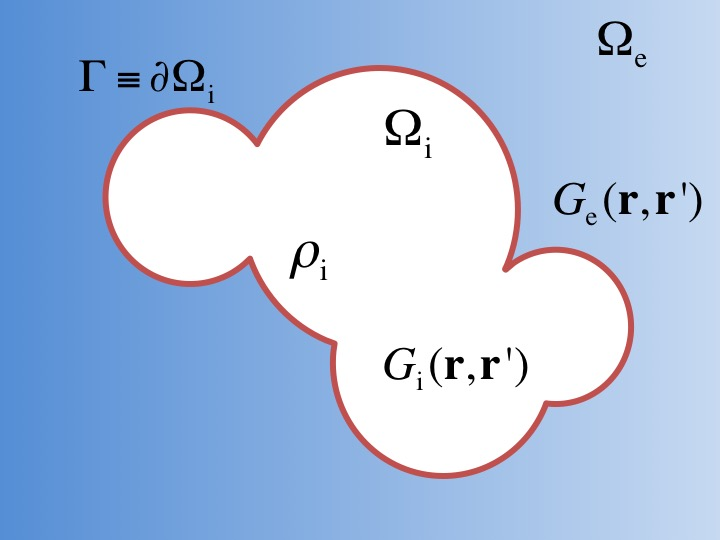
\includegraphics[width=.5\textwidth]{IEF}
  \caption[The physical setting of the polarizable continuum model.]{
  The physical setting of the \ac{PCM}. The molecular solute,
  represented by its, possibly quantum mechanical, charge density
  $\rho_\mathrm{i}$ is enclosed in a \emph{cavity} $\Omegai$.
  The boundary of the cavity $\Gamma\equiv\partial\Omegai$ is a
  continuously differentiable 2-manifold.
  We assume the material properties of the cavity to be those of vacuum,
  hence characterized by the Green's function
  $\Gi=\frac{1}{|\vect{r}-\vect{r}^\prime|}$.
  The cavity is carved out of an infinite, structureless, continuum
  characterized by its Green's function $\Ge$ and fully covering the
  external subdomain $\Omegae$.
  }
  \label{fig:IEF}
\end{figure}

This is a well-known problem in electrostatics~\autocite{Jackson1999, Vanderlinde2005-gf}
and is called a \emph{transmission} problem in the mathematical
literature on \acp{PDE}.~\autocite{Hackbusch1995-uq, Sauter2011-an}
The problem is commonly posed as follows. Given the partition of Euclidean
space $\mathbb{R}^3$ outlined above, find the solution $u(\vect{r})$
to the following set:
\begin{subequations}\label{eq:transmission}
  \begin{align}[left={\empheqlbrace}]
  \Li u &= \nabla^2 u = -4\pi\rhoi \,\, \text{in}\,\, \Omegai \label{eq:internal} \\
  \Le u &= 0 \,\, \text{in}\,\, \Omegae \label{eq:external} \\
  [u] &= \ue - \ui = 0 \,\, \text{on}\,\, \Gamma
  \label{eq:trace-jump} \\
[\partial_L u] &= \partiale u - \partiali u = 0 \,\, \text{on}\,\, \Gamma \label{eq:conormal-jump} \\
|u(\vect{r})| &\leq C \|\vect{r} \|^{-1} \,\,\text{for}\,\,\| \vect{r} \|\rightarrow\infty
\label{eq:radiation}
\end{align}
\end{subequations}
Eqs.~\eqref{eq:trace-jump} and \eqref{eq:conormal-jump}
are the \emph{jump conditions}, expressed in terms of trace operators
for the solution $u$ and its \emph{conormal} derivative.
For notational simplicity, will use the symbols $\partiale$ and $\partiali$
for the latter and only give it in explicit form when needed.
Further mathematical details and technical results on the definition of
function traces and their use in setting up the proper normal and
conormal derivatives can be found in the excellent book by
\citeauthor{Sauter2011-an}.~\autocite{Sauter2011-an}.
The fundamental solutions, or Green's functions, for the elliptic
differential operators $\Li$ and $\Le$ will be denoted by $\Gi$ and
$\Ge$, respectively.
As such the problem is formulated in the so-called \emph{strong} form:
the sought-after solution $u$ has to be at least two times continuously
differentiable.
Moreover, the solution is a function supported over $\mathbb{R}^3$ which
poses challenges to the numerical solution of the problem.
We will take a different approach and reformulate it in terms of
\emph{boundary integral operators}, \ie transform the \acsp{PDE} into a
\ac{BIE}.

The first step is to introduce the relevant boundary integral operators for the
abovementioned transmission problem.
They are three of the four components of the Calder\'on projector.
For any function $v$ in the suitable function space and for $\vect{s}, \vect{s}^\prime \in \Gamma$:
\begin{equation}
\begin{aligned}
  (\bi{S}_\star v)(\vect{s}) &= \int_\Gamma
  G_\star(\vect{s}, \vect{s}^\prime)v(\vect{s}^\prime)\diff \vect{s}^\prime \\
  (\bi{D}_\star v)(\vect{s}) &= \int_\Gamma \partial_{L_\star,\vect{s}}
  G_\star(\vect{s}, \vect{s}^\prime)v(\vect{s}^\prime)\diff \vect{s}^\prime \\
  (\bi{D}^\dagger_\star v)(\vect{s}) &= \int_\Gamma
\partial_{L_\star,\vect{s}^\prime}
  G_\star(\vect{s}, \vect{s}^\prime)v(\vect{s}^\prime)\diff \vect{s}^\prime \\
\end{aligned}
\end{equation}
where $\star$ is a placeholder for the $\mathrm{i}$ or $\mathrm{e}$ subscript.
Our next step is to rewrite the $u$ as the sum of two contributions:
\begin{equation}
  u(\vect{r}) = \esp(\vect{r}) + \xi(\vect{r}) = \int_{\Omegai}
  \frac{\rhoi(\vect{r}^\prime)}{|\vect{r}-\vect{r}^\prime|}
  + \xi(\vect{r})
\end{equation}
the former is the electrostatic potential of $\rhoi$ \emph{in vacuo}
(Newton potential), while the latter is the \emph{reaction} potential.
The reaction potential describes the polarization in the medium.
Moreover, it admits a integral representation as a single-layer
potential:
\begin{equation}
  \xi_\mathrm{i} = \bi{S}_\mathrm{i}\sigma
\end{equation}
where $\sigma$ is the \ac{ASC}, the key quantity in the \acs{PCM}.
As shown by \citeauthor{Cances1998-og}, the \acs{ASC} can be computed
as the \emph{unique} solution to the following integral equation:
\begin{equation}\label{eq:full-IEF}
  \left[ \bi{S}_\mathrm{e}\left(2\pi + \bi{D}^\dagger_\mathrm{i}\right)
  +
  \left(2\pi - \bi{D}_\mathrm{e}\right)\bi{S}_\mathrm{i}
  \right]\sigma =
  -\left[\left(2\pi-\bi{D}_\mathrm{e}\right)
  -\bi{S}_\mathrm{e}\bi{S}_\mathrm{i}^{-1}
  \left(2\pi-\bi{D}_\mathrm{i}\right)
  \right]\esp
\end{equation}
commonly called the \ac{IEF} equation.
The Green's functions for the elliptic differential operators
assume a central role in the boundary integral formulation and make the
\acs{IEF} equation valid for a wide range of external
environments: homogeneous isotropic, ionic and anisotropic
liquids,~\autocite{Cances1998-og}
and systems with interfaces.~\autocite{Corni2002-dr, Frediani2004-er,
Delgado2013-kd, DiRemigio2016-nn}

In the special and very common case of homogeneous and isotropic
environments, \ie regular dielectric materials characterized by a scalar
permittivity $\diel$, the Green's functions are:
\begin{alignat}{2}
  \Ge = \frac{1}{\diel|\vect{r}-\vect{r}^\prime|} = \frac{1}{\diel} \Gi,
  \quad&
  \Gi = \frac{1}{|\vect{r}-\vect{r}^\prime|}
\end{alignat}
yielding the isotropic \acs{IEF} equation:
\begin{equation}\label{eq:isotropic-IEF}
  \bi{R}_\diel\bi{S}\sigma = - \bi{R}_\infty\esp
\end{equation}
where the auxiliary operators:
\begin{alignat}{2}
  \bi{R}_\diel = \left[
  2\pi \left(\frac{\diel+1}{\diel-1}\right) - \bi{D}
  \right],
  \quad&
  \bi{R}_\infty =  \lim_{\diel\rightarrow\infty}\bi{R}_\diel
  = 2\pi-\bi{D}
\end{alignat}
have been introduced.
By letting the $\diel\rightarrow\infty$, one recovers the limiting case
where conductor boundary conditions are imposed. This leads to the
well-known \ac{COSMO} equation:~\autocite{Klamt1993-mj, Cossi2003-xe}
\begin{equation}
  \bi{S}\sigma = - \esp
\end{equation}
\todo[inline]{Mention correction factor $f(\diel)$.}

\section{Detour and Teaser: Weak Formulation of Partial Differential Equations}\label{sec:weak}

From the strong to the weak formulation of \acp{PDE}.\autocite{Ern2004-oo}

\begin{itemize}
  \item Poisson's equation with conductor boundary conditions
        % This is COSMO!
        % This equation makes sense iff \Psi \in \mathcal{C}^2_0(C) (at least)
        % \Psi = 0 \quad \forall \vect{r}\in\partial C
        \begin{equation*}
            \nabla^2\Psi = -4\pi\rho
            % Dirichlet boundary conditions for a conductor
          \quad \Psi \in \mathcolor{ForestGreen}{\mathcal{C}^2_0(C)}
        \end{equation*}
  \item Project onto the space of test functions
        % Project onto the space of test functions
        \begin{equation*}
          \left\{
          \begin{aligned}
            &\text{Seek $\Psi\in\mathcolor{ForestGreen}{V_0}$ such that:}\\
            &(\zeta, \nabla^2\Psi) =
            -4\pi(\zeta, \rho) \quad
            \forall
            \zeta\in\mathcolor{BurntOrange}{\mathcal{C}^\infty_0(C)}
          \end{aligned}
          \right.
        \end{equation*}
  \item Use
    $\eta\nabla^2\gamma = \nabla\cdot(\eta\nabla\gamma) - \nabla\eta\cdot\nabla\gamma$
        % The integral of the first term on the RHS vanishes.
        % It can be shown using Gauss' Theorem and the conductor
        % boundary conditions.
        \begin{equation*}
          \left\{
          \begin{aligned}
            &\text{Seek $\Psi \in \mathcolor{ForestGreen}{H_0^1(C)}$ such that:}\\
            &\mathcolor{Red}{(\nabla\zeta, \nabla\Psi)} =
            \mathcolor{Blue}{-4\pi(\zeta, \rho)} \quad
            \forall \zeta\in \mathcolor{BurntOrange}{H_0^1(C)}
          \end{aligned}
          \right.
        \end{equation*}
\end{itemize}
\begin{equation*}
  \Psi\in \mathcolor{BurntOrange}{H_0^1(C)} = \lbrace f : C \rightarrow
  \mathbb{R} | f \in L^2(C), \nabla f \in L^2(C), f = 0 \forall \vect{s}
  \in\partial C \rbrace
\end{equation*}
\begin{equation}
  \left\{
  \begin{aligned}
    &\text{Seek $\Psi \in V$ such that:}\\
    &\forall \zeta \in V \,\,\,\,\,
    \mathcolor{Red}{a(\zeta, \Psi)} = \mathcolor{Blue}{b(\zeta)}
  \end{aligned}
  \right.
  \label{eq:weak}
\end{equation}

% Hadamard well-posedness definition:
% Problem \eqref{eq:weak} is well-posed if it admits one and only
% one solution and the solution is bounded by the initial data, by
% an a priori estimate (see Ern&Guermond, p.82, Def. 2.1)
\begin{defin}[Well-posedness]\label{def:hadamard}
  The weak problem Eq. \eqref{eq:weak} is \emph{well-posed} if it
  admits one and only one solution and the solution is bounded by
  the initial data by an \emph{a priori} estimate.
\end{defin}
\begin{defin}[Continuity]\label{def:continuity}
  A bilinear form on a normed vector space $V$ is \emph{bounded}, or
  \emph{continuous}, if there is a constant $C$ such that
  $\forall u, v \in V$:
  \[
  a(u, v) \leq C\lVert u\rVert\lVert v\rVert
  \]
\end{defin}
\begin{defin}[Coercivity]\label{def:coercivity}
  A bilinear form on a normed vector space $V$ is \emph{coercive},
  or \emph{elliptic}, if there is a constant $\alpha >0$ such that
  $\forall u \in V$:
  \[
  a(u, u) \geq \alpha\lVert u\rVert^2
  \]
\end{defin}
This implies that no eigenvalue of the linear operator associated
to the bilinear form can be zero, hence that the operator is
invertible!!~\autocite{Ern2004-oo}

% Maybe present connection with Steepest Descent and Conjugate
% Gradient?
% Introduce a suitable vector space, equipped with a norm
% derived from a scalar product.
% The solution belongs to such a vector space, which is
% bigger that in the strong formulation (less constraints on
% the regularity of the solution)
\begin{equation}
  \left\{
  \begin{aligned}
    &\text{Seek $\Psi \in V$ such that:}\\
    &\forall \zeta \in V \,\,\,\,\,
    \mathcolor{Red}{a(\zeta, \Psi)} = \mathcolor{Blue}{b(\zeta)}
  \end{aligned}
  \right.
\end{equation}
\begin{lemma}[Lax--Milgram]
  If the bilinear form $a$ is \emph{continous} and \emph{coercive}
  in $V$, then, for any continuous linear form $b$, Problem~\eqref{eq:weak} is
  \emph{well-posed}.
\end{lemma}
\begin{corollary}[Variational property]
  If the bilinear form is \emph{symmetric} and \emph{positive}
  the unique solution to Problem \eqref{eq:weak} is
  the \emph{unique minimum} on $V$ of the functional:
  \[
  \mathcal{F}(\zeta) = \frac{1}{2}a(\zeta, \zeta) - b(\zeta)
  \]
\end{corollary}

Weak formulation of \acs{BIE}s.\autocite{Hsiao2008-xb}


\section{Numerical Approaches to Boundary Integral Equations}\label{sec:BEM}

Approximability, conformity, consistency and asymptotic consistency
of the approximation setting, $\inf$-$\sup$ condition, Céa's Lemma
and generalized $\inf$-$\sup$ condition.~\autocite{Ern2004-oo,
TesiFilippo}
Additional cavity generators
TsLess~\autocite{Pomelli2004-lb}
DefPol~\autocite{Pomelli1998-ob, Pomelli1999-dc}
FIXPVA~\autocite{Su2009-em}
Other discretization schemes
CSC~\autocite{York1999-xy, Scalmani2010-tw}
SWIG~\autocite{Lange2010-jp, Lange2010-qo, Lange2011-eu}
ddCOSMO and ddPCM~\autocite{Cances2013-jg, Lipparini2013-cy, Lipparini2014-to,
Lipparini2014-fq, Stamm2016-fv}

\todo[inline]{CURRENTLY COPIED VERBATIM FROM THE SPHERICAL GREEN'S
FUNCTION PAPER}

The numerical solution of boundary integral equations, such as the
\acs{IEF}-\acs{PCM}
Eqs.~\eqref{eq:full-IEF-2pi}-\eqref{eq:isotropic-IEF}, can be achieved
by the application of the \ac{BEM}.
A discretization of the molecular cavity
boundary is necessary.~\autocite{Pomelli2007-wq}
The discretization of the
molecular surface into finite elements leads to a corresponding
discretization of both the integral operators and the functions in
Eqs.~\eqref{eq:full-IEF-2pi}-\eqref{eq:isotropic-IEF}.

Different strategies are available to perform the
discretization: the \emph{collocation} or the \emph{Galerkin}
approach.~\cite{Hackbusch1995-uq, Ern2004-oo}
The final result is the transformation of
the original integral equation to a system of linear equations whose
dimension relates to the number of finite elements generated by
discretizing the boundary.  For general integral equations and
discretization schemes, a dense system matrix is obtained. Moreover, the
discretization scheme might not, in general, preserve the symmetry
property of the original integral equation.

In this paper we apply the traditional centroid collocation
method~\autocite{Tomasi2005-vm, Pomelli2007-wq} on the cavity boundary
discretization obtained \emph{via} the GePol
algorithm.~\autocite{Pascual-Ahuir1987-uo, Pascual-Ahuir1990-lp,
Pomelli1998-qp, Pomelli2001-sj, Frediani2004-ua, Pomelli2007-wq}
In this algorithm, the cavity is made of interlocking spheres, not all
of them necessarily centered on the atoms. The surface is then
discretized by means of $N_\mathrm{ts}$ small triangles $\Delta_i$ whose
centroid defines the \emph{collocation point}. Once the centroid is
properly defined, functions and operators are discretized by applying a
one-point quadrature rule in the finite element centroid.
The \acs{IEF}-\acs{PCM} equation is thus recast as:
\begin{equation}
  \vect{q}
  =
  \mat{T}^{-1}\mat{R}\vect{v}.
\end{equation}
$\vect{q}$ and $\vect{v}$ are vectors of dimension $N_\mathrm{ts}$
collecting the values of the \acs{ASC} and \ac{MEP}
at the collocation points.
The matrices representing the boundary integral operators are:
\begin{align}
  \mat{T} &=
  \left(2\pi\mat{I} - \mat{D}_\mathrm{e}\mat{A}\right)\mat{S}_\mathrm{i}
  +\mat{S}_\mathrm{e}\left(2\pi\mat{I} +
  \mat{A}\mat{D}_\mathrm{i}^\dagger\right) \\
  \mat{R} &=
  \left(2\pi\mat{I} - \mat{D}_\mathrm{e}\mat{A}\right) -
  \mat{S}_\mathrm{e}\mat{S}^{-1}_\mathrm{i}\left(2\pi\mat{I}-\mat{D}_\mathrm{i}\mat{A}\right)
\end{align}
$\mat{I}$ is the $N_\mathrm{ts}$-dimensional identity matrix while the
other matrices are defined as:
\begin{alignat}{2}
  &\mat{A} = \mathrm{diag}(\cdots\,\, a_i = \mathrm{area}(\Delta_i)\,\, \cdots) \\
  &S_{ii, \mathrm{i}} = k\sqrt{\frac{4\pi}{a_i}}, \quad
  S_{ij, \mathrm{i}} = \frac{1}{|\vect{s}_i-\vect{s}_j|}\quad (i \neq j) \\
  &D_{ii, \mathrm{i}} = -k\sqrt{\frac{\pi}{a_i}}\frac{1}{R_i}, \quad
  D_{ij, \mathrm{i}} =
  \frac{(\vect{s}_i-\vect{s}_j)\cdot\vect{n}_j}{|\vect{s}_i-\vect{s}_j|^3}\quad (i \neq j) \\
  &S_{ii, \mathrm{e}} = \frac{S_{ii, \mathrm{i}}}{C(\vect{s}_i, \vect{s}_i)} +
        G_\mathrm{img}(\vect{s}_i, \vect{s}_i), \quad
  S_{ij, \mathrm{e}} =
  \frac{1}{C(\vect{s}_i, \vect{s}_j)|\vect{s}_i-\vect{s}_j|} +
  G_\mathrm{img}(\vect{s}_i, \vect{s}_j) \quad (i \neq j) \\
  &D_{ii, \mathrm{e}} = \diel(\vect{s}_i)\left[
  \frac{D_{ii, \mathrm{i}}}{C(\vect{s}_i, \vect{s}_i)}
  -S_{ii, \mathrm{i}}
  \frac{\nabla C(\vect{s}_i,
  \vect{s}_i)\cdot\vect{n}_i}{C^2(\vect{s}_i, \vect{s}_i)}
  +
  \nabla G_\mathrm{img}(\vect{s}_i, \vect{s}_i)\cdot\vect{n}_i
  \right] \\
  &D_{ij, \mathrm{e}} =
  \diel(\vect{s}_j)\left[
  \frac{1}{C(\vect{s}_i, \vect{s}_j)}
  \frac{(\vect{s}_i-\vect{s}_j)\cdot\vect{n}_j}{|\vect{s}_i-\vect{s}_j|^3}
  -\frac{\nabla C(\vect{s}_i,
  \vect{s}_j)\cdot\vect{n}_j}{C^2(\vect{s}_i, \vect{s}_j)}
  \frac{1}{|\vect{s}_i-\vect{s}_j|}
  + \nabla G_\mathrm{img}(\vect{s}_i, \vect{s}_j)\cdot\vect{n}_j
  \right]\quad (i \neq j)
\end{alignat}
in terms of the centroids $\vect{s}_i, \vect{s}_j$, the finite elements
areas and their curvatures $R_i$. The factor $k=1.07$ is introduced to achieve a better precision on the diagonal elements~\cite{Tomasi2005}.

\todo[inline]{CURRENTLY COPIED VERBATIM FROM THE WAVELET PAPER}

Boundary integral equations, such as the \acs{IEF}-\acs{PCM}
Eqs.~\eqref{eq:full-IEF-2pi}-\eqref{eq:isotropic-IEF},
can conveniently be solved numerically by the application of the
\ac{BEM}.
Both the integral operators and the functions on which these act are
defined solely on the boundary of the cavity.

The application of the boundary element method requires that the boundary of
the molecular cavity is discretized by a number of suitable finite elements.
The discretization of the boundary leads to a discretization of the integral
operators. This discretization can be carried out by using either the
\emph{collocation} or the \emph{Galerkin}
approach.~\autocite{Hackbusch1995-uq, Ern2004-oo}
In both cases, the integral equation is transformed to a system of
linear equations whose dimension is related to the number of finite
elements used in the discretization of the boundary.
The resulting system matrix is, in general, a dense matrix. The
boundary element method thus suffers from limitations imposed by the
number of matrix elements to be stored and the memory and time
requirements of solving the resulting linear system.

The use of a wavelet basis in the Galerkin approach has been proven
beneficial in this respect.~\autocite{Harbrecht2004-uo, Dahmen2006-pj,
Harbrecht2006-ug}.
The resulting system matrices are quasi-sparse
and can be further reduced to a sparse form by discarding
negligible entries without considerable loss of precision.

The wavelet boundary element method starts by defining
a sequence of hierarchical trial spaces,
spanned by standard finite element ansatz functions:
\begin{equation}
  \{0\} = V_{-1} \subset V_0 \subset V_1 \subset \ldots
  \subset V_J, \qquad V_j = \Span{\phi_{j,k} : k\in \Delta_{j}}.
\end{equation}
Here, $\Delta_j$ is an index set for the
single-scale basis of the space $V_j$. In the wavelet method,
the trial space $V_j$ is split into the direct sum $V_j = V_{j-1}
\oplus W_j$. The resulting complementary space $W_j$ is called the
wavelet space and is not necessarily orthogonal to $V_{j-1}$.
% It suffices the equation $W_j \cap V_{j-1} = \{0\}$,
Recursive splitting of the trial spaces leads to the wavelet
decomposition $V_j = \bigoplus_{l = 0}^{j} W_l$.

The complementary space is spanned by the wavelet basis:
\begin{equation} W_j =
  \Span{\psi_{j,k}: k \in \Delta_{j+1}
\setminus \Delta_{j}}.
\end{equation}
The choice of this basis turns
out to be very convenient, since we can exploit the compression
technique described by \citeauthor{Dahmen2006-pj} to build up the sparse
system matrix in the wavelet basis directly, avoiding the computation of
non-relevant matrix entries.~\autocite{Dahmen2006-pj}
The \emph{a priori} compression is carried out in two steps. In the
first step, contributions from basis functions sufficiently far away
from each other are discarded. In the following, elements of the matrix
where one wavelet is in the smooth part of the other one are ignored.
The number of relevant matrix entries scales proportional to $O(N_J)$ with
$N_J$ the number of degrees of freedom for a refinement of the geometry
up to level $J$.

In order to understand the compression steps, let us introduce some
notation. Let the \emph{convex hull} of the support of the wavelet $\psi_{j,k}$
be:
\begin{equation}
  \Omega_{j,k} = \conv\hull\left(\supp \psi_{j,k}\right).
\end{equation}
Moreover, let the \emph{singular support} of the wavelet $\psi_{j,k}$ be:
\begin{equation}
  \Omega'_{j,k} = \sing\supp\psi_{j,k}
\end{equation}
It contains all the points in the support where the wavelet is not smooth.
The compression steps are then governed by the following set of
equations
\begin{equation}
  \left[A_J\right]_{\left(j,k\right)\left(j',k'\right)} =
  \begin{cases}
    \quad\quad 0 & \dist(\Omega_{j,k}, \Omega_{j',k'}) > B_{j,j'} \text{ and }j,j' \geq 0, \\
    \quad\quad 0 & \dist(\Omega_{j,k}, \Omega_{j',k'}) \lesssim 2^{-\min\left\{j,j'\right\}} \,\text{and} \\
      & \quad \dist(\Omega'_{j,k}, \Omega_{j',k'}) > B'_{j,j'} \text{ if }j' > j \geq 0, \\
      & \quad \dist(\Omega_{j,k}, \Omega'_{j',k'}) > B'_{j,j'} \text{ if }j > j' \geq 0, \\
    \langle A\psi_{j',k'},\psi_{j,k}\rangle, & \text{otherwise}
  \end{cases}
\label{eq:compression}
\end{equation}
where $\dist(\cdot, \cdot)$ denotes the distance, either between
the bounding boxes of the wavelets or between the singular support and the
bounding box. The first and second conditions represent the first and second
compression step, respectively. The parameters $j,j'$ are the
levels of the wavelets under consideration and the
level-dependent cut-off parameters $B_{j,j'}$ and $B'_{j,j'}$ are given
by
\begin{align*}
  B_{j,j'} &= a \max
  \left\{2^{-\min\left\{j,j'\right\}},
  2^{\frac{J\left(2d^\prime-op\right) -
  \left(j+j'\right)\left(d^\prime+\tilde{d}\right)}{\left(2\tilde{d}+op\right)}}\right\}
  \text{ and }\\ B'_{j,j'} &= a \max
  \left\{2^{-\min\left\{j,j'\right\}},
  2^{\frac{J\left(2d^\prime-op\right) -
\left(j+j'\right)d^\prime-\max\left\{j,j'\right\}\tilde{d}}{\left(\tilde{d}+op\right)}}\right\}
\end{align*}
with $op$ being the order of the integral operator under consideration.
For the first kind integral equation $op = -1$, while $op = 0$ for the second
kind integral equation. The integer $\tilde{d}$ is related to the vanishing
moments of the wavelet basis:
\begin{equation}
  \int \diff\vect{x}\,\,\vect{x}^r \psi_{j,k}(\vect{x}) = 0,
\quad r = 0, \ldots \tilde{d}-1
\end{equation}
In the particular implementation, $\tilde{d}=3$ for the piecewise
constant wavelet basis,  while $\tilde{d}=4$ for the piecewise bilinear
parametrization.~\autocite{Harbrecht2013-hb}
The compression can thus be adjusted by the parameters $a$ and
$d^\prime$:
\begin{equation}\label{eq:param}
  a \geq 1, \quad d < d^\prime < \tilde{d} + op
\end{equation}
where $d$ is the approximation order of the trial spaces $V_j$:
$d=1, 2$ for piecewise constant and
piecewise bilinear ansatz functions, respectively.
Note that, if the interaction between two wavelets, $\psi_{j,k}$ and $\psi_{j',k'}$, on
level $j$ and $j'$ is neglected in the system matrix, all other
interactions between wavelets resulting from the refinement of
$\psi_{j,k}$ and $\psi_{j',k'}$ can also be ignored. Thus, the
compression pattern of the system matrix is calculated
hierarchically starting from the coarsest level.

Once the compressed system matrix is assembled, we arrive at a sparse
system matrix in the wavelet basis which can be compressed further by
leaving out the sufficiently small elements. This post-processing step
is governed by the rule
\begin{equation}
  \left[A_J\right]_{\left(j,k\right)\left(j',k'\right)}
  \begin{cases}
    \quad\quad 0 & \text{if } |\left[ A_J \right]_{\left(j,k\right)\left(j',k'\right)}| \leq \epsilon_{j,j'}\\
    \left[A_J\right]_{\left(j,k\right)\left(j',k'\right)}, & \text{otherwise,}
  \end{cases}
  \label{eq:aposteriori}
\end{equation}
where the coefficients $\epsilon_{j,j'}$ are given by
\begin{equation}
%\epsilon_{j,j'} = b\min \left\{2^{-|j-j'|}, 2^{-\left(2J-\left(j+j'\right)\right)\frac{2d^\prime-op}{2\tilde{d}+op}}\right\} 2^{J\,op}2^{-2d^\prime\left(J-\frac{j+j'}{2}\right)},
  \epsilon_{j,j'} = b\min \left\{2^{-|j-j'|}, 2^{-\left(2J-\left(j+j'\right)\right)\frac{2d^\prime-op}{2\tilde{d}+op}}\right\} 2^{-2d^\prime\left(J-\frac{j+j'}{2}\right)}
\end{equation}
with the \emph{a posteriori} compression parameter $b < 1$.

\section[Variational Formulation of Classical Polarizable Models]{
Above and Beyond: Classical Polarizable Models within a Variational Formulation}
\label{sec:variational}

Variational functional for implicit models, \acs{PCM} in this
case:~\autocite{Lipparini2010-be, Lipparini2011-aj, Lipparini2016-mo}
\begin{equation}
 U_\mathrm{PCM} = \frac{1}{2}\scalprod{\sigma}{\PCM\sigma} + \scalprod{\esp}{\sigma}
\end{equation}

Variational functional for explicit models,~\autocite{Lipparini} could be
MMpol~\autocite{Curutchet} or PE~\autocite{Steindal, Kongsted, Olsen} or
FQ~\autocite{Rick1994-mn, Rick1995-wu, Rick1996-om, Lipparini}:
\begin{equation}
  U_\mathrm{MM} = \frac{1}{2}\kappa\MM\kappa + \kappa\zeta
\end{equation}

The PCM equations will be written in the ``complete basis'' meaning that
we will introduce the usual \ac{BEM} discretization
at the very end of the derivation. In other words, we will be working
with the exact integral equation and not with its discretized
counterpart. As a consequence, the apparent surface charge $\sigma$ and
the electrostatic potential $\esp$ will have a \emph{continuous}
dependence on a ``cavity surface'' index $\vect{s}$. Whenever a
charge-potential product is present it is then to be interpreted as the
\emph{surface integral}, i.e. the scalar product in the suitable,
infinite-dimensional vector space on the cavity boundary $\Gamma$. The
following shorthand notation will be adopted:
\begin{equation}
 \sigma\esp = \scalprod{\sigma}{\esp}
\end{equation}

Coupled implicit/explicit polarization energy
functional:~\autocite{Lipparini}
\begin{equation}\label{eq:pcm-mm-functional}
  U_\mathrm{pol} =
   \frac{1}{2}\sigma\PCM\sigma + \sigma\esp
 + \frac{1}{2}\kappa\MM\kappa + \kappa\zeta
 + \sigma\bi{X}\kappa
\end{equation}
where one has:
\begin{equation}
  \sigma\MMPCM\kappa = \kappa\MMPCM^\dagger\sigma
\end{equation}
and $\MMPCM$ is the implicit/explicit interaction kernel. This is
charge/dipole or charge/charge interaction kernel for the MMpol and
\ac{PE} models
or the \ac{FQ} model, respectively.
The global minimum of the convex functional is found by differentiating
it with respect to the variational degrees of freedom, \ie{} the
\acl{ASC} (\acs{ASC}) density $\sigma$ and the classical point
charges/dipoles $\kappa$. This leads to the coupled equations:
\begin{align}
  \PCM\sigma + \esp + \MMPCM\kappa &= 0 \\
  \MM\kappa  + \zeta + \MMPCM^\dagger\sigma &= 0
\end{align}
or in the commonly found matrix form:
\begin{equation}
  \begin{pmatrix}
    \PCM & \MMPCM \\
    \MMPCM^\dagger & \MM
  \end{pmatrix}
  \begin{pmatrix}
   \sigma \\
   \kappa
  \end{pmatrix}
  =
  -
  \begin{pmatrix}
   \esp \\
   \zeta
  \end{pmatrix}
\end{equation}
Finally, let us re-express the equations above in a "supermatrix"
formalism:
\begin{equation}
  U_\mathrm{pol} =
  \frac{1}{2}{}^t\p\V\p + {}^t\p\s
\end{equation}
where:
\begin{alignat}{3}
  \p =
  \begin{pmatrix}
    \sigma \\
    \kappa
  \end{pmatrix},
  \quad&
  \s =
  \begin{pmatrix}
   \esp \\
   \zeta
  \end{pmatrix},
  \quad&
  \V =
  \begin{pmatrix}
    \PCM & \MMPCM \\
    \MMPCM^\dagger & \MM
  \end{pmatrix}
\end{alignat}
and the ${}^t\p$ symbol denotes the transposed supervector $\p$.
The supermatrix form will prove particularly useful in the following
derivations.

\todo[inline]{PUT REFERENCES HERE!!!}
The variational formulation offers a series of advantages.
The classical energy functional:
\begin{equation}
  U_\mathrm{pol} =
   \frac{1}{2}\sigma\PCM\sigma + \sigma\esp
 + \frac{1}{2}\kappa\MM\kappa + \kappa\zeta
 + \sigma\bi{X}\kappa
\end{equation}
renders itself to a straightforward physical interpretation. In the
three bilinear terms, \ie{} the ones mediated by an interaction
operator, we can identify the self-interaction of the classical
polarization with itself, be it purely implicit:
$\frac{1}{2}\sigma\PCM\sigma$, purely explicit
$\frac{1}{2}\kappa\MM\kappa$ or mixed $\sigma\MMPCM\kappa$.
These terms are positive definite and give rise to an unfavorable
contribution, which is counterbalanced by the linear terms. These terms
mediate the interaction between the induced polarization and the
inducing fields: $\esp$ and $\zeta$. While $\esp$ is quite clearly the
\acl{MEP} (\acs{MEP}), $\zeta$ can either be the molecular electric
field (MMpol and \acs{PE} models) or again the \acs{MEP} (\acs{FQ} model).
In any case, both will be determined by the quantum mechanical molecular
charge density and can thus be formulated as expectation values of
one-electron operators. Eventually, this achieves the coupling between
the classical -- $\sigma$ and $\kappa$ -- and
the quantum mechanical variational degrees of freedom.

\todo[inline]{Mention the classical equivalent of the Hellmann--Feynman
theorem and why it is particularly useful in formulating response
theory.}
